%Version 2.1 April 2023
% See section 11 of the User Manual for version history
%
%%%%%%%%%%%%%%%%%%%%%%%%%%%%%%%%%%%%%%%%%%%%%%%%%%%%%%%%%%%%%%%%%%%%%%
%%                                                                 %%
%% Please do not use \input{...} to include other tex files.       %%
%% Submit your LaTeX manuscript as one .tex document.              %%
%%                                                                 %%
%% All additional figures and files should be attached             %%
%% separately and not embedded in the \TeX\ document itself.       %%
%%                                                                 %%
%%%%%%%%%%%%%%%%%%%%%%%%%%%%%%%%%%%%%%%%%%%%%%%%%%%%%%%%%%%%%%%%%%%%%

\documentclass[sn-basic,pdflatex]{sn-jnl}

%%%% Standard Packages
%%<additional latex packages if required can be included here>

\usepackage{graphicx}%
\usepackage{multirow}%
\usepackage{amsmath,amssymb,amsfonts}%
\usepackage{amsthm}%
\usepackage{mathrsfs}%
\usepackage[title]{appendix}%
\usepackage{xcolor}%
\usepackage{textcomp}%
\usepackage{manyfoot}%
\usepackage{booktabs}%
\usepackage{algorithm}%
\usepackage{algorithmicx}%
\usepackage{algpseudocode}%
\usepackage{listings}%
%%%%

%%%%%=============================================================================%%%%
%%%%  Remarks: This template is provided to aid authors with the preparation
%%%%  of original research articles intended for submission to journals published
%%%%  by Springer Nature. The guidance has been prepared in partnership with
%%%%  production teams to conform to Springer Nature technical requirements.
%%%%  Editorial and presentation requirements differ among journal portfolios and
%%%%  research disciplines. You may find sections in this template are irrelevant
%%%%  to your work and are empowered to omit any such section if allowed by the
%%%%  journal you intend to submit to. The submission guidelines and policies
%%%%  of the journal take precedence. A detailed User Manual is available in the
%%%%  template package for technical guidance.
%%%%%=============================================================================%%%%

%% Per the spinger doc, new theorem styles can be included using built in style, 
%% but it seems the don't work so commented below
%\theoremstyle{thmstyleone}%
\newtheorem{theorem}{Theorem}%  meant for continuous numbers
%%\newtheorem{theorem}{Theorem}[section]% meant for sectionwise numbers
%% optional argument [theorem] produces theorem numbering sequence instead of independent numbers for Proposition
\newtheorem{proposition}[theorem]{Proposition}%
%%\newtheorem{proposition}{Proposition}% to get separate numbers for theorem and proposition etc.

%% \theoremstyle{thmstyletwo}%
\theoremstyle{remark}
\newtheorem{example}{Example}%
\newtheorem{remark}{Remark}%

%% \theoremstyle{thmstylethree}%
\theoremstyle{definition}
\newtheorem{definition}{Definition}%



\raggedbottom




% tightlist command for lists without linebreak
\providecommand{\tightlist}{%
  \setlength{\itemsep}{0pt}\setlength{\parskip}{0pt}}





\begin{document}


\title[Lab Notebook]{Ordinal Pattern Analysis for Early Bearing Fault
Detection and Classification in Rotating Machinery}

%%=============================================================%%
%% Prefix	-> \pfx{Dr}
%% GivenName	-> \fnm{Joergen W.}
%% Particle	-> \spfx{van der} -> surname prefix
%% FamilyName	-> \sur{Ploeg}
%% Suffix	-> \sfx{IV}
%% NatureName	-> \tanm{Poet Laureate} -> Title after name
%% Degrees	-> \dgr{MSc, PhD}
%% \author*[1,2]{\pfx{Dr} \fnm{Joergen W.} \spfx{van der} \sur{Ploeg} \sfx{IV} \tanm{Poet Laureate}
%%                 \dgr{MSc, PhD}}\email{iauthor@gmail.com}
%%=============================================================%%

\author*[1]{\fnm{Rasika} \sur{Dilhani} \dgr{MSc}}\email{\href{mailto:rasidilhani@gmail.com}{\nolinkurl{rasidilhani@gmail.com}}}

\author[1]{\fnm{Alejandro} \sur{Author} }



  \affil*[1]{\orgdiv{School of Mathematics and
Statistics}, \orgname{Victoria University of
Wellington}, \orgaddress{\city{Wellington}, \country{New
Zealand}, \postcode{6012}, \state{}, \street{}}}

\abstract{This research aims to identify perturbations in machines using
time series data, where detecting chaotic patterns is notably
challenging. Bandt and Pompe proposed looking at time series from the
perspective of ordinal patterns to develop fast and automated methods
for extracting qualitative information from nonlinear time series. They
developed the idea of permutation entropy to measure the complexity of a
system underlying a time series, taking into account the ordinal
patterns that represent the variations in a time series. Only one aspect
of the ordinal structure of a time series is revealed by the permutation
entropy. Here we show how to use the real-valued data set to extract all
ordinal information.}

\keywords{ordinal patterns, permutation entropy, bearing fault data}



\maketitle

\section{Introduction}\label{sec1}

Bearings are critical components in rotating machinery, yet their
demanding operating conditions, which involve high loads and impacts,
often lead to various faults. These faults can cause significant
downtime, costly maintenance, and even complete machine failure.
Therefore, early and accurate detection and classification of bearing
faults are essential to ensure operational reliability and minimize
maintenance costs.

Traditional fault detection methods primarily rely on analyzing physical
parameters and trends using techniques such as vibration analysis,
thermal monitoring, and current signature analysis. While these methods
have proven effective, they can be susceptible to noise and often
require substantial computational resources. Ordinal pattern analysis
has emerged as a promising alternative, offering a robust and
computationally efficient approach to analyzing time series data.

At its core, ordinal pattern analysis transforms continuous time series
data into a sequence of ordinal patterns that represent the order
relationships among data points within a specified time window. This
approach effectively captures the fundamental dynamics of the signal in
a way that is inherently robust to noise and distortions. By analyzing
these patterns, it becomes possible to identify subtle changes in system
behavior that may indicate the presence of a fault.

This study investigates the application of ordinal pattern analysis for
the early detection and classification of bearing faults, focusing on
common fault types such as ball defects, outer race defects, and inner
race defects. Using a publicly available dataset from the Case Western
Reserve University Bearing Data Center, we demonstrate the effectiveness
of ordinal patterns in distinguishing between healthy and faulty bearing
conditions.

Our research explores the advantages of ordinal pattern analysis in
detecting changes in system dynamics associated with faults. By
identifying alterations in the frequency and recurrence of specific
temporal patterns, this technique can reveal subtle indicators of
developing faults. Furthermore, unlike some traditional methods limited
to linear systems, ordinal pattern analysis can effectively detect
faults in complex, non-linear systems, broadening its applicability.

While traditional methods often rely on specialized sensors and data
acquisition systems, ordinal pattern analysis has the potential to
achieve comparable results using simpler time series data, underscoring
its potential for broader adoption. We investigate the sensitivity of
ordinal pattern analysis to subtle changes in system dynamics,
particularly in complex systems, where its strengths may be most
pronounced.

Our goal is to establish ordinal pattern analysis as a viable and
advantageous tool for bearing fault diagnosis, contributing to
advancements in predictive maintenance technologies and promoting more
efficient and reliable operation of rotating machinery.

\section{Literature Review}\label{sec2}

<<<<<<< HEAD
In the study conducted by \citet{WOS:000312724900101}, an enhanced
approach is introduced to detect bearing faults using high-frequency
resonance, which improves the precision and reliability of fault
diagnosis in mechanical systems. The study demonstrates that this
refined methodology effectively identifies early bearing abnormalities,
marking a significant advancement over conventional diagnostic
techniques. Additionally, \citet{WOS:000301688000008} present a new
technique for fault identification that uses an adaptive rank-order
morphological filter to categorize patterns in one-dimensional signals.
This approach increases the accuracy and robustness of fault diagnosis
by effectively filtering and identifying signal irregularities.
Furthermore, \citet{WOS:000303039300034} proposes a method for early
fault detection in machinery by analyzing truncated vibration signals
through Shannon wavelet spectrum analysis. This technique enhances the
detection of emerging faults, thereby improving the prognostic
maintenance of equipment.

\citet{WOS:000345844100102} discuss a prototype FPGA implementation that
uses machine learning to convert analog signals into concise feature
representations. This prototype employs an event-based methodology to
=======
In the study conducted by researchers \citet{WOS:000312724900101}, an
enhanced approach is introduced to detect bearing faults through the
utilization of high-frequency resonance, resulting in improved precision
and dependability in diagnosing faults within mechanical systems. The
investigation illustrates that this refined methodology adeptly
recognizes initial bearing abnormalities, representing a significant
progression compared to conventional diagnostic techniques. The article
by \citet{WOS:000301688000008} presents a new technique for fault
identification which employs an adaptive rank-order morphological filter
to categorize patterns in one-dimensional signals. This strategy
enhances the precision and resilience of fault diagnosis by proficiently
sifting through and pinpointing signal irregularities. Furthermore,
\citet{WOS:000303039300034} propose an approach for early fault
detection in machinery by scrutinizing truncated vibration signals using
Shannon wavelet spectrum analysis. This method heightens the detection
of emerging faults, thereby enhancing the prognostic maintenance of
equipment.

\citet{WOS:000345844100102} discusses a prototype FPGA implementation
that uses machine learning to convert analog signals into concise
feature representations. It employs an event-based methodology to
>>>>>>> fbcf525c5ded840d987846476241d9360b1302a6
enhance the efficiency and accuracy of signal processing across various
applications. \citet{WOS:000396580800080} explore the use of a dedicated
hierarchy of neural networks for evaluating bearing degradation, thereby
improving the precision and reliability of diagnosing the condition and
remaining operational life of bearings in machinery. Additionally,
\citet{WOS:000320835800016} combine multifractal detrended fluctuation
analysis with the Mahalanobis distance criterion to enhance the fault
diagnosis of rolling bearings, leading to improved diagnostic accuracy
and providing efficient, validated methods for early fault detection in
industrial settings.

An additional intriguing research study detailed in the publication
\citet{WOS:000360994300029} introduces a diagnostic technique for
rolling element bearings grounded in the concept of active perception.
This method is based on the examination of the dynamic interactions
between the bearing and its surrounding environment. Noteworthy
discoveries include the capability of the approach to precisely evaluate
the bearing's condition by integrating perceptual cues and responses,
thereby enhancing fault detection and predictive maintenance strategies.
\citet{WOS:000343577703075} present a fault diagnosis approach for
rolling element bearings that makes use of Empirical Mode Decomposition
(EMD) in conjunction with Discrete Fourier Domain Analysis (DFDA). This
technique effectively isolates and scrutinises fault-related
characteristics in vibration signals, thereby enhancing the accuracy and
dependability of bearing condition diagnosis. The utilisation of a
signal-based triangular structuring element for mathematical
morphological analysis, along with the application of this method to
enhance fault diagnosis in rolling element bearings through the
effective processing and interpretation of vibration signal features,
was discussed in the publication \citep{WOS:000334316700001}. Moreover,
a hybrid CEEMD-EMD approach for fault detection in rolling bearings,
which combines Complete Ensemble Empirical Mode Decomposition with Noise
(CEEMD) and traditional Empirical Mode Decomposition (EMD), has been
developed in the manuscript by \citet{WOS:000412752200052} to enhance
the precision of vibration signal analysis and augment fault detection
capabilities.

<<<<<<< HEAD
In their paper, \citet{WOS:000335959500009} put forth a methodology for
bearing fault detection that employs compressive measurements of
vibration signals to efficiently detect faults, thereby enhancing
diagnostic accuracy while reducing the data processing load. A
distinctive technique for feature extraction, founded upon the crossover
attributes of nonlinear data, is employed to facilitate enhanced fault
diagnosis in rotary machinery through the effective identification of
critical patterns in intricate signal data \citep{WOS:000338603900013}.
The application of Self-Organising Maps (SOMs) has proven effective in
diagnosing motor bearing faults through the classification of complex
vibration data. Furthermore, approaches based on fast nonlocal means and
envelope spectra have been shown to contribute to improving the accuracy
of fault diagnosis. Furthermore, a low-dimensional compressed
measurement strategy enhances the efficiency of fault detection, while a
Bayesian inference technique guided by a smoothness index enables the
precise identification of various bearing faults through the analysis of
anti-symmetric real Laplace wavelet parameters
\citep{WOS:000380543400119, WOS:000348309400067, WOS:000354607100016, WOS:000350998800016}.
A novel machine fault diagnosis method utilising the Statistical Local
Linear Embedding Algorithm (S-LLE) has been developed. This is an LLE
extension that employs fault class labels to enhance feature extraction,
dimensionality reduction and pattern recognition. This is achieved by
mapping high-dimensional vibration signal vectors, which have been
processed through the time domain, into a low-dimensional space. The
aforementioned techniques are then combined with frequency-domain and
empirical mode decomposition (EMD) to create a low-dimensional space,
which has been demonstrated to outperform PCA, LDA, and LLE for rapid
fault classification. This is evidenced by the analysis of rolling
bearing error signals, which have been shown to achieve superior error
classification performance compared to conventional methods
\citep{WOS:000361788200068}. The combination of wavelet packet
decomposition with multi-scale permutation entropy has the potential to
accurately detect bearing faults by utilising hidden Markov models
\citep{WOS:000362513400031}. The results demonstrate that this approach
significantly enhances the accuracy of fault detection in comparison to
traditional methods, achieving greater precision in the identification
of fault types and their severity. The integration of wavelet packet
decomposition with multiscale permutation entropy serves to enhance the
reliability of fault diagnosis systems, thereby rendering it a valuable
technique for the purposes of predictive maintenance in industrial
=======
The authors of the paper \citet{WOS:000335959500009} propose a
methodology for bearing fault detection that utilizes compressive
measurements of vibration signals to efficiently detect faults,
enhancing diagnostic accuracy while reducing the data processing load. A
unique technique for feature extraction, based on the crossover
characteristics of nonlinear data, is applied to enhance fault diagnosis
in rotary machinery by effectively identifying critical patterns in
complex signal data \citep{WOS:000338603900013}. Self-Organizing Maps
(SOMs) are successful in diagnosing motor bearing faults through the
classification of complex vibration data, while approaches based on fast
nonlocal means and envelope spectra contribute to improving fault
diagnosis accuracy. Moreover, a low-dimensional compressed measurement
strategy boosts fault detection efficiency, and a Bayesian inference
technique guided by a smoothness index enables precise identification of
various bearing faults by analyzing anti-symmetric real Laplace wavelet
parameters
\citep{WOS:000380543400119, WOS:000348309400067, WOS:000354607100016, WOS:000350998800016}.
A novel machine fault diagnosis method using the Statistical Local
Linear Embedding Algorithm (S-LLE), an LLE extension leveraging fault
class labels to enhance feature extraction, dimensionality reduction,
and pattern recognition by mapping high-dimensional vibration signal
vectors---processed through time-domain, frequency-domain, and empirical
mode decomposition (EMD)---into a low-dimensional space, which
outperforms PCA, LDA, and LLE for swift fault classification, as
validated by rolling bearing error signals, thereby achieving superior
error classification performance over conventional methods
\citep{WOS:000361788200068}. The combination of wavelet packet
decomposition with multi-scale permutation entropy exhibits potential in
accurately detecting bearing faults, utilizing hidden Markov models
\citep{WOS:000362513400031}. Results demonstrate that this approach
significantly improves fault detection accuracy compared to traditional
methods, achieving higher precision in identifying fault types and their
severity. Integrating wavelet packet decomposition with multi-scale
permutation entropy enhances the reliability of fault diagnosis systems,
making it a valuable technique for predictive maintenance in industrial
>>>>>>> fbcf525c5ded840d987846476241d9360b1302a6
applications.

\citet{WOS:000365686400021} introduced a new feature extraction
technique, Window Marginal Spectrum Clustering (WMSC), for diagnosing
faults in roller element bearings (REBs). This method combines the
Hilbert-Huang Transform (HHT) and Support Vector Machines (SVM) to
enhance classification accuracy and robustness against Gaussian white
noise. Experimental results using datasets from the Case Western Reserve
University (CWRU) Bearing Data Center demonstrate that WMSC outperforms
traditional methods. \citet{WOS:000366534900022} presented ``The
Diagnostic Line,'' a novel criterion for monitoring the condition of
rotating machinery, which aims to improve the accuracy and reliability
of machinery health diagnoses. A comparative analysis using CWRU data
was conducted to evaluate various diagnostic techniques and establish a
standard reference for bearing fault diagnosis
\citep{WOS:000357230900007}. \citet{WOS:000385104500001} proposed an
improved Wavelet Total Variation Denoising (W-TVD) technique for
mechanical fault diagnosis, effectively filtering noise and enhancing
fault detection accuracy. Findings show that this approach significantly
outperforms traditional denoising methods. Research on fault diagnosis
in industrial rotating equipment, utilizing permutation entropy, signal
processing techniques, and a multi-output neuro-fuzzy classifier,
demonstrates effective identification of fault types and severity
levels. Results indicate that combining permutation entropy for feature
extraction with signal processing clarifies and distinguishes fault
signatures, while the neuro-fuzzy classifier achieves high accuracy in
multi-class fault identification. This integrated approach enhances
diagnostic reliability and performance, offering a robust solution for
real-time fault detection in industrial machinery \citep{Rajabi2022}.
\citet{WOS:000392016300001} elaborated on an adapted kernel marginal
Fisher analysis (MKMFA) technique for feature extraction and
dimensionality reduction to improve bearing fault diagnosis accuracy. By
extracting critical low-dimensional features and using a K-nearest
neighbor classifier, this approach demonstrates superior performance
compared to alternative methods in identifying diverse bearing faults.

<<<<<<< HEAD
Signal analysis of vibrations is an effective approach for diagnosing
mechanical faults. However, identifying defects in their early stages is
challenging due to noise from other components
\citep{WOS:000369301600001, WOS:000367992900001}. These studies
introduce a new methodology that combines time-domain analysis with
adaptive fuzzy C-means clustering.

\citet{WOS:000366765500038} presents an innovative technique for
assessing machinery damage using manifold learning principles to compute
subspace distances. \citet{WOS:000379556300014} explores the use of
Multivariate Empirical Mode Decomposition (MEMD) in diagnosing faults in
rolling bearings, demonstrating its effectiveness in enhancing fault
detection by thoroughly analyzing complex, multidimensional signal data.

\citet{WOS:000391229300006} proposes a methodology for diagnosing faults
in rolling element bearings by integrating Multifractal Theory with Gray
Relation Theory, designed to improve the accuracy and reliability of
fault detection and analysis, ultimately enhancing diagnostic outcomes.
\citet{WOS:000426819400027} investigates a new approach for analyzing
vibration signals in rolling bearings, which combines dual-entropy,
Holder coefficient, and Gray Relation Theory. This integration aims to
boost the precision and reliability of diagnostics, achieving higher
levels of fault detection efficiency.
=======
Signal analysis of vibrations is a significantly efficient approach for
diagnosing mechanical faults. However, the identification of defects in
their early stages poses a challenge due to the presence of noise from
components \citep{WOS:000369301600001, WOS:000367992900001}. These
studies introduce a fresh methodology that merges time domain analysis
with adaptive fuzzy C-means clustering. \citet{WOS:000366765500038}
introduces an innovative technique for assessing machinery damage,
utilizing manifold learning principles to compute subspace distances.
\citet{WOS:000379556300014} presents the utilization of Multivariate
Empirical Mode Decomposition (MEMD) in diagnosing rolling bearings'
faults. It demonstrates the effectiveness of this method in improving
fault detection by thoroughly analyzing complex, multidimensional signal
data. \citet{WOS:000391229300006} proposes a methodology for diagnosing
faults in rolling element bearings by integrating Multifractal Theory
and Gray Relation Theory. This integration is designed to improve the
precision and reliability of fault detection and analysis, ultimately
enhancing diagnostic results. A new approach for examining vibration
signals in rolling bearings, which combines dual-entropy, Holder
coefficient, and Gray Relation Theory is studied by
\citet{WOS:000426819400027}. This integration aims to improve the
efficiency of fault detection and analysis by leveraging these methods
to achieve higher levels of precision and reliability in diagnostics.
>>>>>>> fbcf525c5ded840d987846476241d9360b1302a6

\citet{WOS:000398818700108} discusses the Shock Pulse Index (SPI) and
its application in diagnosing faults in rolling element bearings,
highlighting SPI's effectiveness in detecting and analyzing bearing
condition and performance issues. Results demonstrate that SPI provides
accurate fault detection and is a valuable tool for monitoring and
diagnosing bearing health.

\citet{WOS:000404415000016} examines fault diagnosis for rolling
bearings under variable conditions using visual cognition techniques.
Findings indicate that visual cognition methods significantly enhance
the ability to identify and assess bearing faults in changing
operational environments.

\citet{WOS:000401109400020} introduces sparse discriminant manifold
projections for bearing fault diagnosis, utilizing advanced
dimensionality reduction techniques to improve fault detection and
classification accuracy. Results show that this method effectively
identifies bearing faults by capturing essential discriminative features
while minimizing noise and irrelevant data.

\citet{WOS:000419006900041} presents a fault detection method for
analyzing rolling bearings' vibration signals using the Symplectic
Entropy method. This method assesses the complexity and patterns in
vibration data, enhancing fault identification accuracy. Findings
confirm that this approach effectively detects faults by providing a
robust measure of signal irregularities and anomalies.

\citet{WOS:000416794600016} propose a method for extracting incipient
fault features in rolling bearings using an autocorrelation function
impulse harmonic-to-noise ratio index, combined with Singular Value
Decomposition (SVD) and the Teager Energy Operator. Results indicate
that this approach effectively identifies early-stage faults by
amplifying subtle signal anomalies amidst noise.

\citet{WOS:000484465800028} present a bearing fault diagnosis method
combining autoencoders with Particle Swarm Optimization (PSO) and
Support Vector Machines (SVM). This approach leverages autoencoders for
feature extraction and dimensionality reduction, while PSO optimizes SVM
parameters, resulting in improved diagnostic accuracy and robustness for
bearing fault identification.

\citet{WOS:000477760600037} introduce an optimized resolution
coefficient algorithm for the Gray Relation Classifier to enhance
classification accuracy. This algorithm refines the resolution
coefficients, improving the classifier's ability to distinguish between
classes, leading to more precise fault diagnosis and analysis.

\citet{WOS:000477760600061} proposes a subtle feature extraction
algorithm using an improved fractal box-counting dimension method. This
method enhances the detection of fine-grained signal features by
refining fractal dimension calculations, resulting in better
identification and analysis of subtle signal patterns.

A novel rolling bearing fault detection method based on the Empirical
Wavelet Transform (EWT) effectively decomposes vibration signals into
components that highlight fault-related features, thereby enhancing
detection accuracy and robustness in identifying bearing faults
\citep{WOS:000467079500501}.

\citet{WOS:000459864800144} introduce a bearing fault detection method
that combines Empirical Mode Decomposition (EMD) with Random Forest.
This approach analyzes vibration signals under varying operational
conditions by decomposing them into intrinsic mode functions and
classifying fault patterns, leading to improved detection accuracy and
reliability.

\citet{WOS:000458657500187} critically examine the importance of feature
extraction and selection in diagnosing bearing defects, emphasizing that
effective feature extraction and selection are essential for improving
diagnostic accuracy and reliability by identifying the most relevant
characteristics in vibration signals.

An online health status estimation technique for rolling bearings based
<<<<<<< HEAD
on vibration signals focuses on real-time monitoring and analysis to
evaluate bearing condition. Research shows that this method effectively
assesses health status through continuous vibration data analysis to
identify and predict potential faults \citep{WOS:000452922000015}.

\citet{WOS:000453413600001} present an automatic classification approach
for bearing faults using deep learning methods. This approach employs
neural networks to analyze and categorize fault patterns in vibration
signals, leading to enhanced accuracy and efficiency in fault detection
and diagnosis.

\citet{WOS:000452819600235} introduce a method for early fault diagnosis
in bearings using the Empirical Wavelet Transform (EWT) combined with
energy entropy. By analyzing vibration signals with detailed frequency
decomposition and measuring the distribution of signal energy, this
method improves the accuracy of early fault identification.

Another study by \citet{WOS:000450745100001}, along with
\citet{WOS:000449334500118}, introduces a technique for detecting faults
=======
on vibration signals, with a focus on real-time monitoring and analysis
for evaluating bearing condition. It is shown in the research that this
method effectively assesses health status through continuous evaluation
of vibration data to identify and predict potential faults
\citep{WOS:000452922000015}. An automatic classification approach for
bearing faults is presented by \citet{WOS:000453413600001}, utilizing
deep learning methods that employ neural networks to examine and
categorize fault patterns present in vibration signals. This leads to
enhanced accuracy and efficiency in the detection and diagnosis of
bearing faults. \citet{WOS:000452819600235} introduces a method for
early fault diagnosis in bearings using Empirical Wavelet Transform
(EWT) in conjunction with energy entropy. By analyzing vibration signals
with detailed frequency decomposition and measuring the distribution of
signal energy, this method improves the identification accuracy of early
faults. Another study \citet{WOS:000450745100001} and
\citet{WOS:000449334500118} introduces a technique for detecting faults
>>>>>>> fbcf525c5ded840d987846476241d9360b1302a6
in rolling element bearings that involves segmenting vibration signals
and applying wavelet analysis with deep neural networks. This method
improves fault detection by segmenting signals into meaningful parts for
enhanced accuracy, using wavelet transforms for feature extraction, and
employing deep neural networks for clustering and categorization,
resulting in more precise identification of bearing faults.

<<<<<<< HEAD
The study by \citet{WOS:000440977000032} introduces a technique for
extracting bearing fault features using autoregressive coefficients,
Linear Discriminant Analysis (LDA), and Support Vector Machines (SVM)
under varying operational conditions. This combination of methods
enhances fault detection by accurately identifying and categorizing
fault features, even in changing operational settings.

\citet{WOS:000434717400001} propose a unique diagnostic approach for
rolling element bearings, integrating Noise-Assisted Multivariate
Empirical Mode Decomposition (MEMD) with a Functional Neural Fuzzy
Network. This approach uses MEMD for effective feature extraction and
the neural fuzzy network for precise fault classification, resulting in
improved diagnostic precision and reliability.

\citet{WOS:000426284100001} present a fault diagnosis method for rolling
bearings that employs Modified Local Fisher Discriminant Analysis (LFDA)
and Empirical Mode Decomposition (EMD) along with sensitive feature
selection. The goal is to enhance fault detection by accurately
extracting and analyzing critical features from vibration signals.

\citet{WOS:000539546400083} detail an initial fault diagnosis technique
for rolling bearings that combines Empirical Wavelet Transform (EWT)
with Spectral Kurtosis. This method focuses on detecting initial faults
through refined frequency analysis with EWT and highlighting abnormal
signal features using Spectral Kurtosis, leading to improved early fault
detection and diagnostic accuracy.

\citet{hakim2023systematic} introduce an enhanced similarity-based
=======
The present study of \citet{WOS:000440977000032} introduces a technique
for extracting bearing fault features using autoregressive coefficients,
Linear Discriminant Analysis (LDA), and Support Vector Machines (SVM) in
varying operational conditions. These methods are combined to improve
fault detection by accurately identifying and categorizing fault
features even amidst changing operational settings. A unique diagnostic
approach for rolling element bearings is proposed, which integrates
Noise-Assisted Multivariate Empirical Mode Decomposition (MEMD) with a
Functional Neural Fuzzy Network \citep{WOS:000434717400001}. This
integration utilizes MEMD to extract features effectively and the neural
fuzzy network for precise fault classification, resulting in enhanced
diagnostic precision and reliability. \citet{WOS:000426284100001}
presents a fault diagnosis method for rolling bearings that utilizes
Modified Local Fisher Discriminant Analysis (LFDA) and Empirical Mode
Decomposition (EMD) along with sensitive feature selection. The
objective is to enhance fault detection by extracting and examining
critical features from vibration signals with improved accuracy and
discrimination. \citet{WOS:000539546400083} details an initial fault
diagnosis technique for rolling bearings that merges Empirical Wavelet
Transform (EWT) with Spectral Kurtosis. The focus is on detecting
initial faults through refined frequency analysis with EWT and
highlighting abnormal signal features using Spectral Kurtosis, leading
to improved early fault detection and diagnostic accuracy. Another study
of \citet{hakim2023systematic} introduces an enhanced similarity-based
>>>>>>> fbcf525c5ded840d987846476241d9360b1302a6
modeling approach for classifying failures in rotating machines. By
applying advanced similarity measures to better match failure patterns,
this method significantly improves diagnostic precision. Results
indicate that it outperforms traditional classification techniques,
achieving higher accuracy and reliability in failure detection.
Additionally, a comprehensive review is provided on fault diagnosis
methods for rolling bearings that utilize deep learning and transfer
learning techniques.

\citet{WOS:000345844100102} discuss a prototype FPGA implementation that
uses machine learning to convert analog signals into concise feature
representations. This implementation employs an event-based methodology
to enhance the efficiency and accuracy of signal processing across
various applications.

\citet{WOS:000396580800080} explore a hierarchical neural network model
to assess bearing degradation, aiming to improve the accuracy and
reliability of diagnosing machinery bearing conditions and estimating
remaining operational life.

\citet{WOS:000320835800016} enhance rolling bearing fault diagnosis by
combining multifractal detrended fluctuation analysis with the
Mahalanobis distance criterion. This approach leads to improved
diagnostic accuracy and provides efficient, validated methods for early
fault detection in industrial settings.

An additional intriguing study by \citet{WOS:000360994300029} introduces
a diagnostic technique for rolling element bearings based on the concept
of active perception. This method examines the dynamic interactions
between the bearing and its surroundings. Key findings include the
approach's ability to accurately assess bearing condition by integrating
perceptual cues and responses, thereby enhancing fault detection and
predictive maintenance strategies.

\citet{WOS:000343577703075} present a fault diagnosis approach for
rolling element bearings that combines Empirical Mode Decomposition
(EMD) with Discrete Fourier Domain Analysis (DFDA). This technique
effectively isolates and examines fault-related characteristics in
vibration signals, resulting in improved accuracy and reliability in
diagnosing bearing conditions.

\citet{WOS:000334316700001} discuss the use of a signal-based triangular
structuring element for mathematical morphological analysis to enhance
fault diagnosis in rolling element bearings. This approach enables
effective processing and interpretation of vibration signal features.

Furthermore, \citet{WOS:000412752200052} propose a hybrid CEEMD-EMD
strategy for fault detection in rolling bearings, merging Complete
Ensemble Empirical Mode Decomposition with Noise (CEEMD) and traditional
Empirical Mode Decomposition (EMD). This hybrid method enhances the
precision of vibration signal analysis and improves fault detection
capabilities.

\citet{WOS:000335959500009} propose a methodology for bearing fault
detection that utilizes comprehensive vibration signal measurements to
efficiently detect faults, enhancing diagnostic accuracy while reducing
data processing requirements.

\citet{WOS:000338603900013} apply a unique feature extraction technique
based on the crossover properties of nonlinear data to improve fault
diagnosis in rotating machinery by effectively identifying critical
patterns in complex signal data.

Research shows that self-organizing maps (SOMs) successfully diagnose
engine bearing faults by classifying complex vibration data, while
methods based on fast non-local averages and envelope spectra further
improve diagnostic accuracy. Additionally, a low-dimensional compressed
measurement strategy enhances error detection efficiency, and a Bayesian
inference technique based on a smoothness index precisely identifies
various bearing errors through the analysis of anti-symmetric real
Laplace wavelet parameters
\citep{WOS:000380543400119, WOS:000348309400067, WOS:000354607100016, WOS:000350998800016}.

Recent studies have focused on advanced methodologies for bearing fault
diagnosis using vibration signals. Statistical locally linear embedding
has been suggested as a powerful technique for dimensionality reduction
and feature extraction, outperforming conventional methods like PCA and
LDA \citep{WOS:000361788200068}.

\citet{WOS:000362513400031} combine wavelet packet decomposition with
multi-scale permutation entropy and hidden Markov models, showing that
this approach significantly improves fault detection accuracy compared
to traditional methods. It achieves higher precision in identifying
fault types and severity levels. Integrating wavelet packet
decomposition with multi-scale permutation entropy further enhances the
reliability of fault diagnosis systems, making it a valuable technique
for predictive maintenance in industrial applications.

\citet{WOS:000365686400021} introduce a new feature extraction technique
called Window Marginal Spectrum Clustering (WMSC) for diagnosing faults
in roller element bearings (REBs). This method employs the Hilbert-Huang
Transform (HHT) and Support Vector Machines (SVM) to enhance
classification accuracy and robustness against Gaussian white noise.
Experimental results using datasets from the Bearing Data Center at Case
Western Reserve University (CWRU) demonstrate that WMSC outperforms
conventional methods.

Additionally, \citet{WOS:000366534900022} present ``The Diagnostic
Line,'' a novel criterion for monitoring the condition of rotating
machinery, aimed at improving the accuracy and reliability of machinery
health diagnostics.

A comparative analysis conducted by \citet{WOS:000357230900007}, using
data from Case Western Reserve University, evaluated various diagnostic
techniques and established a standard reference for bearing fault
diagnosis. The current study builds upon this investigation,
incorporating the same dataset for further examination using a novel
time series model.

Furthermore, an innovative two-stage strategy has been developed that
uses permutation entropy for fault detection, combined with wavelet
packet transform, envelope analysis, and neuro-fuzzy classification for
fault isolation. This approach demonstrates improved diagnostic
performance compared to existing techniques
\citep{WOS:000385104500001, Rajabi2022}, contributing to more precise
and effective bearing fault diagnosis in rotating industrial machines.

Another study introduces an adapted kernel marginal Fisher analysis
(MKMFA) technique for feature extraction and dimensionality reduction to
enhance the accuracy of bearing fault diagnosis. By extracting critical
low-dimensional features and employing a K-nearest neighbor classifier,
this method outperforms alternative approaches in identifying various
bearing defects \citep{WOS:000392016300001}.

Vibration signal analysis is a highly efficient approach for diagnosing
mechanical faults. However, identifying early-stage defects remains
challenging due to noise from other components
\citep{WOS:000369301600001, WOS:000367992900001}. This study introduces
a new methodology that combines time-domain analysis with adaptive fuzzy
C-means clustering. It uses nine standard parameters in the time domain
to construct characteristic vectors and improves clustering by
optimizing five specific parameters: variance, RMS, kurtosis, skewness,
and crest factor. Research demonstrates the method's sensitivity in
detecting even minor errors.

Additionally, an innovative fault diagnosis technique for rolling
bearings is developed by integrating Multifractal Detrended Fluctuation
Analysis (MFDFA) with Alpha Stable Distribution (ASD) functions. This
integration enhances fault detection capabilities by improving
sensitivity and reliability.

The article by \citet{WOS:000366765500038} presents an innovative
technique for assessing machine damage using various learning principles
to calculate subspace distances. This method enhances the accuracy and
responsiveness of damage assessment by employing advanced dimensionality
reduction techniques.

\citet{WOS:000379556300014} explore the use of Multivariate Empirical
Mode Decomposition (MEMD) for diagnosing rolling bearing defects,
demonstrating its effectiveness in improving fault detection through
in-depth analysis of complex, multidimensional signal data.

\citet{WOS:000391229300006} propose a methodology for diagnosing defects
in rolling bearings by integrating multifractal theory with Gray
Relation Theory. This integration is designed to improve the precision
and reliability of fault detection and analysis, ultimately enhancing
diagnostic outcomes.

\citet{WOS:000426819400027} introduce a new approach for investigating
vibration signals in rolling bearings that combines dual entropy, Holder
coefficient, and Gray Relation Theory. This integration aims to improve
the efficiency of fault detection and analysis by leveraging these
methods to achieve higher levels of precision and reliability in
diagnosis.

\citet{WOS:000398818700108} discuss the Shock Pulse Index (SPI) and its
application in diagnosing failures in rolling bearings, highlighting
SPI's effectiveness in detecting and analyzing bearing health and
performance issues. Results indicate that SPI enables accurate fault
detection and serves as a valuable tool for monitoring and diagnosing
bearing condition.

The current study also examines the diagnosis of rolling bearing faults
under variable conditions using visual detection techniques. The goal is
to show how visual analysis can enhance fault detection and diagnosis
accuracy. Findings indicate that visual detection methods significantly
improve the ability to identify and assess bearing defects in dynamic
operational environments \citep{WOS:000404415000016}.

\citet{WOS:000401109400020} introduce sparse discriminant manifold
projections for bearing fault diagnosis, employing advanced
dimensionality reduction techniques to improve fault detection and
classification accuracy. Results show that this method effectively
identifies bearing defects by capturing key distinguishing features
while minimizing noise and irrelevant data.

In a related study, \citet{WOS:000419006900041} present a fault
detection method for rolling bearing vibration signals using the
symplectic entropy method. This method analyzes the complexity and
patterns of vibration data to improve fault detection accuracy. Results
demonstrate that this approach effectively detects faults by providing a
robust measure of signal irregularities and anomalies.

\citet{WOS:000416794600016} propose a method for extracting incipient
fault features in rolling bearings using an autocorrelation function
impulse harmonic noise ratio index, combined with Singular Value
Decomposition (SVD) and the Teager Energy Operator. Results show that
this approach effectively identifies early-stage faults by enhancing the
detection of subtle signal anomalies amid noise.

\citet{WOS:000484465800028} present a method for bearing fault diagnosis
that combines autoencoders with particle swarm optimization (PSO) and
support vector machines (SVM). This approach uses autoencoders for
feature extraction and dimensionality reduction, while PSO optimizes SVM
parameters, resulting in improved diagnostic accuracy and robustness in
bearing fault identification.

\citet{WOS:000477760600037} introduce an optimized resolution
coefficient algorithm for the Gray Relation Classifier, designed to
improve classification accuracy by enhancing the algorithm's ability to
distinguish between classes with refined resolution coefficients. This
results in more precise fault diagnosis.

\citet{WOS:000477760600061} propose an algorithm for extracting subtle
signal features using an improved fractal box-counting dimension method.
This method refines the fractal dimension calculation, leading to better
detection and analysis of fine-grained signal features, resulting in
improved identification of subtle signal patterns.

\citet{WOS:000467079500501} propose a novel rolling bearing defect
detection method based on empirical wavelet transform (EWT), which
effectively decomposes vibration signals into components that highlight
defect-related features, thereby enhancing detection accuracy and
robustness in identifying bearing defects.

\citet{WOS:000459864800144} present a bearing fault detection method
that combines Empirical Mode Decomposition (EMD) with Random Forest to
effectively analyze vibration signals under varying operating
conditions. This approach decomposes signals into intrinsic mode
functions and classifies fault patterns, resulting in improved detection
accuracy and reliability.

\citet{WOS:000458657500187} critically examine the importance of feature
extraction and selection in diagnosing bearing defects, emphasizing that
effective feature extraction and selection are crucial for enhancing
diagnostic accuracy and reliability by identifying the most relevant
features from vibration signals.

Another study by \citet{WOS:000452922000015} employs an online approach
to estimate rolling bearing health status based on vibration signals,
with a focus on real-time monitoring and analysis. The study
demonstrates that this approach effectively estimates health status by
continuously evaluating vibration data to detect and predict potential
faults.

An automatic bearing defect classification method utilizes deep learning
techniques, leveraging neural networks to analyze and classify defect
patterns from vibration signals. This approach enhances the accuracy and
efficiency of bearing defect detection and diagnosis
\citep{WOS:000453413600001}.

An early fault diagnosis method for bearings uses empirical wavelet
transform (EWT) combined with energy entropy to improve the detection of
incipient faults. By analyzing vibration signals with refined frequency
decomposition and measuring signal energy distribution, this method
achieves higher accuracy in early fault detection
\citep{WOS:000452819600235}.

\citet{WOS:000450745100001}; \citet{WOS:000449334500118} present a
rolling bearing defect detection method that combines vibration signal
segmentation with wavelet analysis and deep neural networks. This
approach improves fault detection by dividing signals into meaningful
segments for greater accuracy, using wavelet transforms for feature
extraction, and applying deep neural networks for clustering and
classification. This results in more precise identification and
categorization of bearing faults.

\citet{WOS:000440977000032} introduce a method for extracting bearing
fault features using autoregressive coefficients, Linear Discriminant
Analysis (LDA), and Support Vector Machines (SVM) under varying
operating conditions. By combining these techniques, the method enhances
fault detection by accurately extracting and classifying fault features
in changing operational environments.

\citet{WOS:000434717400001} propose a novel rolling bearing fault
diagnosis method that integrates noise-assisted multivariate empirical
mode decomposition (MEMD) with a functional fuzzy neural network. This
approach leverages noise-assisted MEMD for effective feature extraction
and the fuzzy neural network for precise fault classification, resulting
in improved diagnostic accuracy and robustness.

\citet{WOS:000426284100001} introduce a method for diagnosing rolling
bearing defects that combines modified Fisher Local Discriminant
Analysis (LFDA) with Empirical Mode Decomposition (EMD) and sensitive
feature selection. This method aims to improve defect detection by
extracting and analyzing critical features from vibration signals with
enhanced accuracy and discrimination.

\citet{WOS:000539546400083} present an early diagnosis method for
rolling bearings that integrates Empirical Wavelet Transform (EWT) with
spectral kurtosis. This approach focuses on detecting incipient faults
by using EWT for refined frequency analysis and spectral kurtosis to
highlight abnormal signal features, leading to improved early fault
detection and diagnostic accuracy.

\citet{WOS:000426986200020} propose an improved similarity-based
modeling approach for classifying failures in rotating machinery. This
approach enhances fault classification accuracy and effectiveness by
leveraging advanced similarity metrics to better match fault patterns,
resulting in higher diagnostic accuracy. Results indicate that this
method significantly outperforms traditional classification techniques,
achieving greater accuracy and reliability in fault detection.

\citet{hakim2023systematic} provide a comprehensive review of rolling
bearing failure diagnosis methods that utilize deep learning and
transfer learning, offering a detailed taxonomy, overview, and
application of these techniques. The review addresses current challenges
and limitations, recommending areas for future research. It highlights
that deep learning and transfer learning approaches have notably
improved fault diagnosis accuracy and robustness but also points to
challenges such as the need for larger, more diverse datasets and the
difficulty of generalizing models across varying operating conditions.
The review suggests that addressing these challenges could further
enhance the effectiveness and applicability of advanced diagnostic
methods.

\subsection{Permutation Entropy}\label{permutation-entropy}

Permutation entropy is a widely used feature for quantifying the
complexity and randomness of time series data. It can also be described
as a measure of a signal's proximity to white noise. This concept was
introduced by Christoph Bandt and Bernd Pompe in 2002
\citep{PhysRevLett.88.174102}. The primary goal of developing this
method was to create a robust and invariant approach for analyzing
complex signals across various fields, including finance, social
systems, climate science, physics, physiology, and neuroscience.

The complexity measure is computed from the probabilities of ordinal
patterns and has been applied to tasks such as analyzing bearing fault
recordings at different machine speeds. The convergence behavior of the
asymptotic variance of permutation entropy to its limit distribution was
studied by \citep{REY2024115481}. These findings enable tests for
comparing the underlying dynamics of two time series. We apply these
tests to distinguish uniform white noise in bearing fault data.

A key advantage of this approach is its ability to plot a point with
coordinates of entropy and statistical complexity within a closed
manifold. The position of this point reveals structural information
about the underlying dynamics that generated the time series data, as we
introduced.

For notational simplicity, we consider a real-valued time series of
length \(N=n+D-1; D\ge2\) is an integer known as the embedding
dimension. We denote this time series as \textbf{\(x\)}
\(= (x_1, x_2, ..., x_{n+D-1})\). For \(t=1, 2, …,n,\) let
\(s_t = (x_t,x_{t+1},…,x_{t+D-1})\) represent an overlapping window of
\(D\) consecutive values in \(x\). Assume that each of these values is
distinct. Then, map each subsequence \(s_t\) to a symbol \(\pi_t\)
uniquely determined by the indexes that sort
\((x_t, x_{t+1}, ..., x_{t+D-1})\); this is the ordinal pattern of
\(s_t\). This process, known as ``Bandt--Pompe Symbolization'' or
``Ordinal Pattern Transformation,'' converts the time series
\textbf{\(x\)} into a sequence of symbols
\(\pi=(\pi_1, \pi_2, ..., \pi_n)\). Each symbol \(\pi_j\) can take one
of \(D!\) possible values:
\(\pi_j \in \Pi=\{\pi^{(1)}, \pi^{(2)}, ..., \pi^{(D!)}\}\). The
probability that the pattern \(\pi^{(i)}\) appears in the sequence
\textbf{\(\pi\)} is denoted by \(q_i,\) for \(i=1,2, ..., D!\).

The sequence of patterns is invariant to monotonically increasing
transformations of \textbf{\(x\)} and is less sensitive to outliers than
descriptors that rely on the original values \citep{chagas2022white}.
These two properties make ordinal patterns effective for signal analysis
and interpretation \citep{amigo2023ordinal}. Ordinal patterns are
computed by constructing a histogram of the proportions of symbols in
\textbf{\(\pi\)}.

Let \(p=(p_1 ,p_2 ,... p_k)\) be a probability vector of size \(k\). The
Shannon entropy based on the \(p\) vector is defined as follows:
\begin{equation}
S^{(s)}[p]=-\sum_{i=1}^{k}{p_i \log p_i}
\end{equation}

\subsection{Ordinal Patterns}\label{ordinal-patterns}

In this section, we provide a brief overview of the methodology based on
ordinal patterns proposed by Bandt and Pompe
\citep{PhysRevLett.88.174102}. We use a real-valued time series,
represented by the vector \(x = (x_1, x_2, ..., x_{n+D-1})\), where
\(n\) and \(D\ge 2\) are positive integers, to illustrate the concept.

Consider an overlapping window \(s_t=(x_t, x_{t+1}, ..., x_{t+D-1})\) of
\(D\) consecutive, distinct values in \(x\). Let
\(\Pi=\{\pi^{(1)}, \pi^{(2)}, ..., \pi^{(D!)}\}\) represent the set of
labeled permutations, or symbols, of the indices \(0,1,...,D-1\),
corresponding to the possible ordinal patterns defined as follows: Given
\(t \in \{1,2,...,n\},\) the subsequence \(s_t\) is of type
\(\pi^{(i)}=(i_1, i_2, ..., i_D),\) if
\(x_{t+i_1}\le x_{t+i_2} \le ...\le x_{t+i_D}.\) In cases of tied data,
order is determined by the sequential appearance of repeated values. For
example, when \(D=3,\) the subsequence \(s_t=(4,2,4)\) is of type
\((1,0,2)\). Thus, from the time series \(x,\) we obtain a sequence of
symbols or ordinal patterns \(\pi=(\pi_1, \pi_2, ..., \pi_n),\) where
\(\pi_j \in \Pi\) for \(j=1,2,...,n.\)

The underlying dynamics of the time series determine the ordinal pattern
probability vector, represented as \(V = (q_1,q_2, ..., q_{D!}),\) where
\(q_i,\) indicates the relative frequency of the pattern \(\pi^{(i)}\)
in the sequence of ordinal patterns, for \(i=1,2,...,D!.\)

This calculation operates by examining neighboring values within a
predefined embedding dimension \(D,\) assigning them to a corresponding
ordinal pattern. The number of possible patterns depends on the
embedding dimension \(D\), with \(|\pi_D|=D!\), where \(\pi_D\),
contains all possible ordinal patterns. For example, if \(D=3\) then
\(|\pi_3|=3!=6,\) corresponding to the patterns
\(\{123, 132, 213, 231, 312, 321\}\) as illustrated in @ref(fig:fig\_1).

\begin{figure}
<<<<<<< HEAD
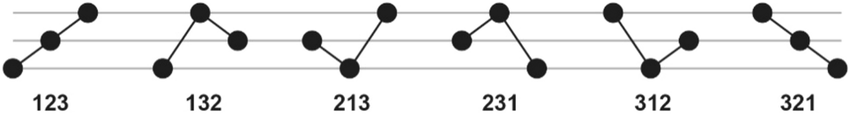
\includegraphics{./fig_1} \caption{The number of possible patterns for the embedding dimension 3}\label{fig:fig_1}
=======
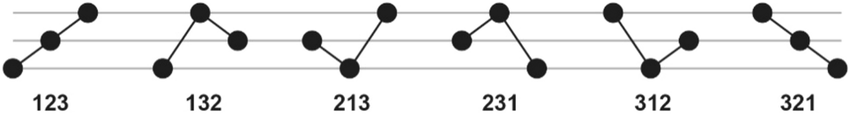
\includegraphics[width=11.81in,]{./fig_1} \caption{The number of possible patterns for the embedding dimension 3}\label{fig:unnamed-chunk-1}
>>>>>>> fbcf525c5ded840d987846476241d9360b1302a6
\end{figure}

\section{Methodology}\label{Methodology}

The data were obtained from the Bearing Data Center and the seeded fault
test data at the Case Western Reserve University, School of Engineering.
The dataset includes ball bearing test data for normal bearings, as well
as single-point defects on the drive end and fan end. Data were
collected at rates of 12,000 and 48,000 data points per second for the
drive-end bearing tests, and at 12,000 data points per second for the
fan-end bearing tests. Each file includes motor rotational speed,
drive-end vibration data, and fan-end vibration data. The variable names
in each file indicate the following:

\begin{itemize}
  \item DE - drive end accelerometer data
  \item FE - fan end accelerometer data
  \item BA - base accelerometer data
  \item time - time series data
  \item RPM - rpm during testing 
\end{itemize}

For ease of use, the data were categorized as Normal Baseline Data, 12k
Drive End Bearing Fault Data, 48k Drive End Bearing Fault Data, and Fan
End Bearing Fault Data. The normal baseline data include four motor load
levels: 0, 1, 2, and 3, with approximate motor speeds provided in RPM
(1797, 1772, 1750, and 1730). The 12k Drive End, 48k Drive End, and 12k
Fan End bearing data follow the same motor load levels and speeds. This
research aims to identify faulty machines using the separate time series
data.

This study explores the use of ordinal pattern analysis for the early
detection and classification of bearing faults, focusing on common fault
types such as ball, outer race, and inner race defects. Using a publicly
available dataset from the Case Western Reserve University Bearing Data
Center, we demonstrate the effectiveness of ordinal patterns in
distinguishing between healthy and faulty bearing conditions.

This research aims to identify faulty machines. Each data file consists
of two time series, which we examine using ordinal patterns. We
introduce distance as a measure of similarity between segments based on
their ordinal structure. With specific embedding dimensions, this metric
can be used to distinguish faulty machines. We apply permutation entropy
for rolling bearing fault diagnosis and show that embedding dimensions
from 3 to 6 effectively separate faulty machines. Some machines exhibit
white noise, which lies near the lower and upper boundaries. The
complexity plane is used to analyze the results, confirming that
dimension 5 yields the best outcomes.

Examples of time series data are shown as follows.

\begin{figure}
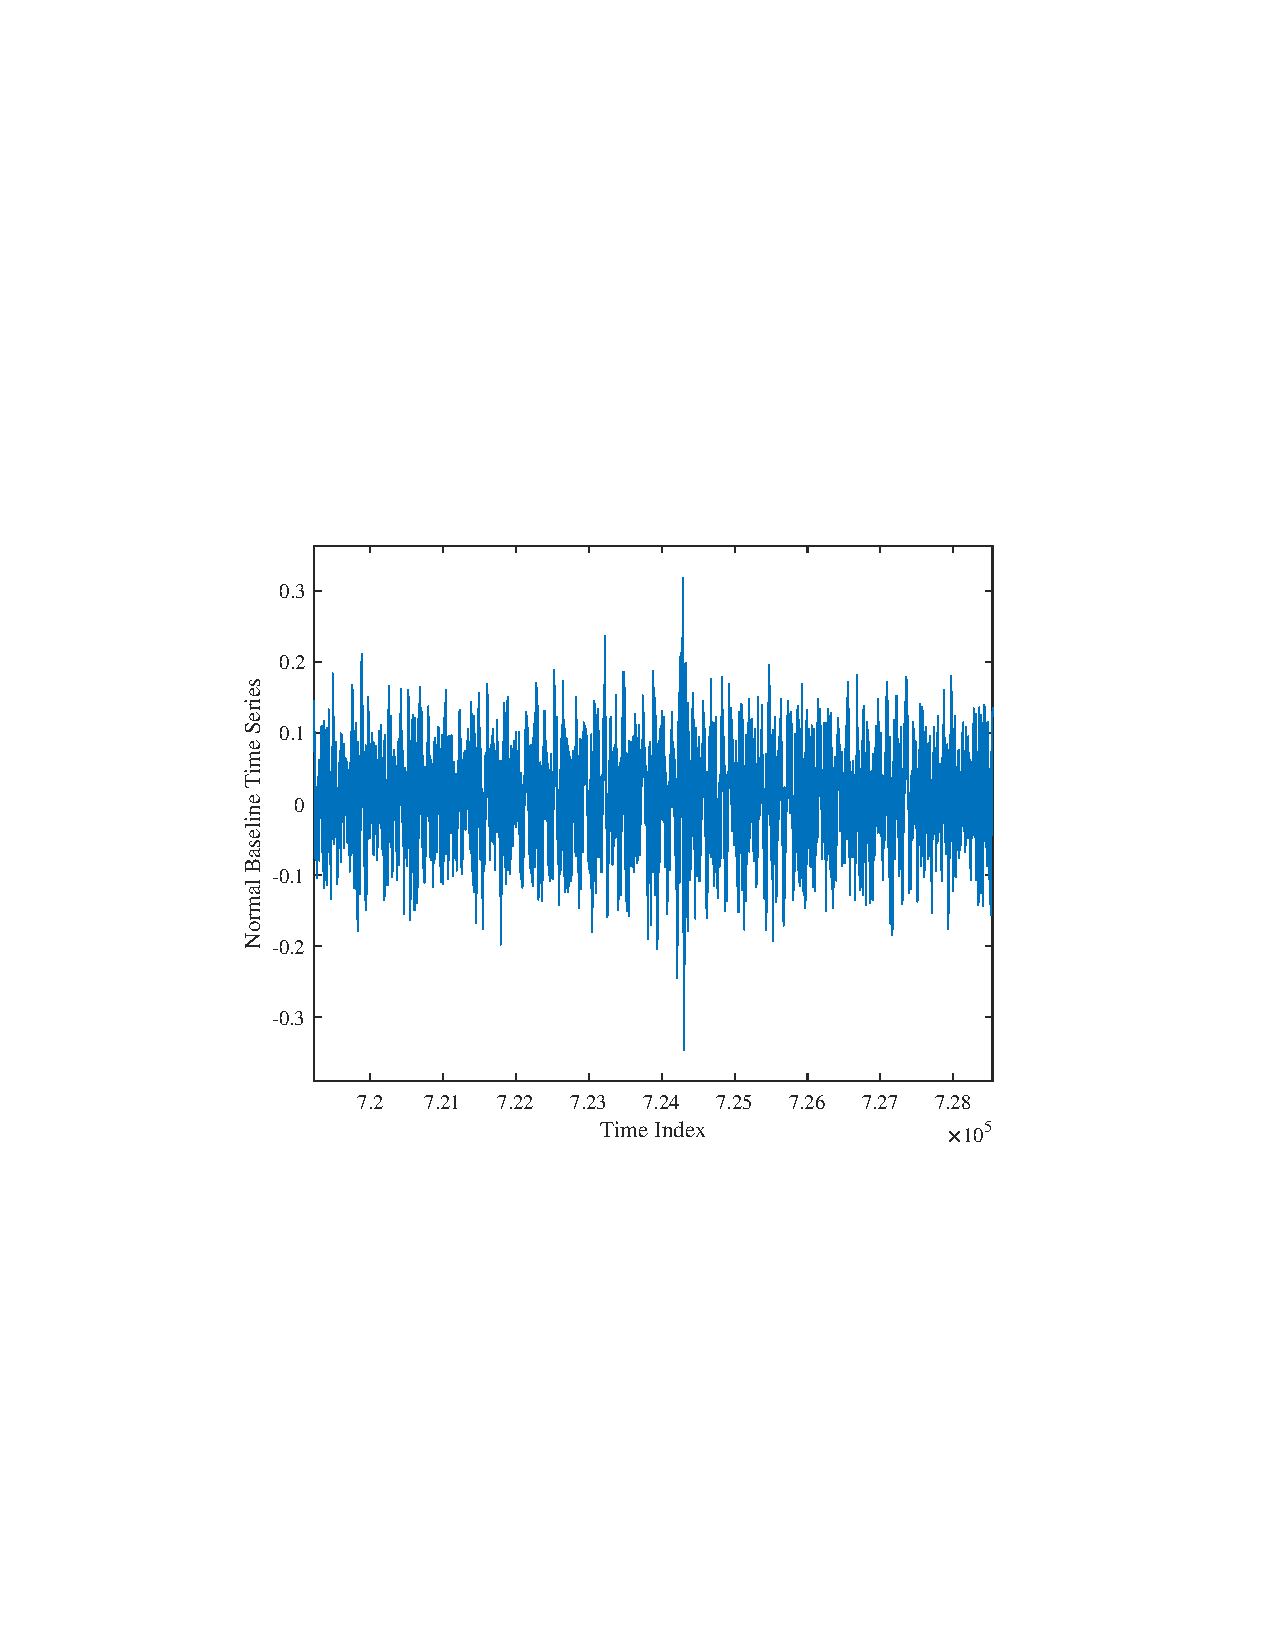
\includegraphics[width=0.5\linewidth,]{./normalbaselinetimeSeriesDE} \caption{The number of possible patterns for the embedding dimension 3}\label{fig:unnamed-chunk-1}
\end{figure}

\begin{figure}
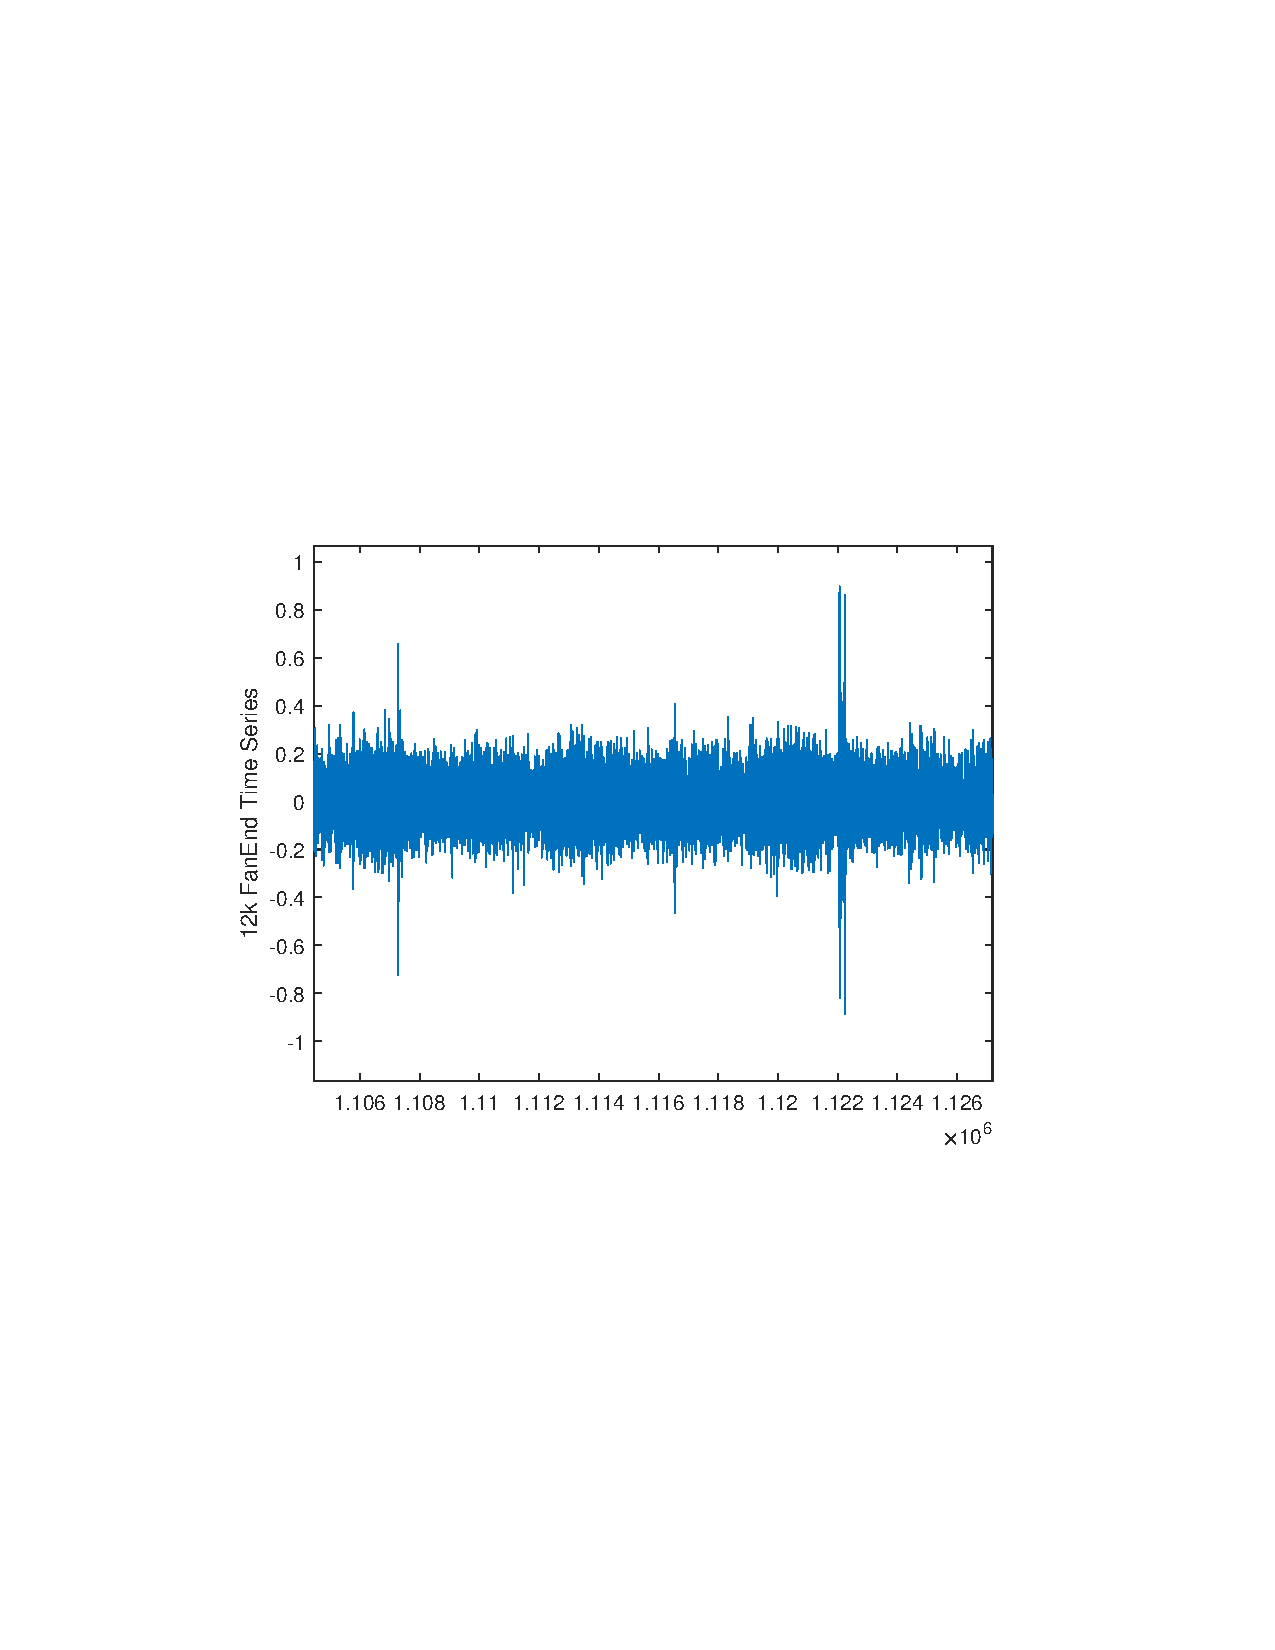
\includegraphics[width=0.5\linewidth,]{./fanend12kDE} \caption{The number of possible patterns for the embedding dimension 3}\label{fig:unnamed-chunk-2}
\end{figure}

Figure 2 shows the DE, FE and BA time series for engine loads 0, 1, 2
and 3. From these time series it is not possible to identify the faulty
machines. However, Figures 3 and 4 show the normal baseline DE time
series for a motor load of 0 and the accelerometer time series data at
the 12,000 fan end for a motor load of 0. The graph is clear and it can
be seen that it is failure time series data is about time series.
However, it is difficult to separate the exact machine type and other
characteristics of the data. The main idea of this research work is to
identify perturbation machines using the various time series data given
above. First, time series data were analyzed and then the method
described by \citet{REY2024115481} used the StatOrdPatt package to
analyze the data. Next, the probability distribution of the ordinal
pattern was considered and the entropy permutation entropy was
calculated accordingly. Based on the entropy of each time series data,
the entropy complexity level was considered to distinguish the faulty
machines.

\section{Results}\label{Results}

Permutation entropy guarantees the separation of error machines. With
this experimental result, we can see that the embedding dimensions from
3 to 6 result in separate error machines. We see that the machines form
clusters, but also that they have individual signatures. The following
graphic shows the lower and upper bounds of the points in entropy
complexity level for embedding dimensions between 3 and 6 for engine
load 0,1,2 and 3. The points of the time series in the \(H×C\) plane as
well as the confidence intervals for their Shannon entropies are taken
into account.

\bibliography{BearingFaultDiagnosis.bib}


\end{document}
